\section{Model performance with Train/Test sets}
\label{ch:traintest}

To be more rigorous about judging model performance, and to avoid overfitting, we can fit our models using a \textit{training set} and evaluate it on new data in the \textit{test set}.

\subsection{Summary of model parameters and results}
Below is a summary of the parameters for the mathematical models, also located in the plots in the body of the report

\import{./}{Chapters/Ireland-mathmodelpars.tex}
\import{./}{Chapters/Italy-mathmodelpars.tex}
\import{./}{Chapters/United States-mathmodelpars.tex}

Below is a summary of results of the applied model for the primary date range for the training set (at least 4 weeks). The test set is then the following fourteen days of cases.

\import{./}{Chapters/Ireland-summarydf.tex}
\import{./}{Chapters/Italy-summarydf.tex}
\import{./}{Chapters/United States-summarydf.tex}

The moving average is only here for comparison and usually outperforms all other models.

\subsection{Base and Periodic models}
\begin{figure}[H]
\minipage{0.48\textwidth}
  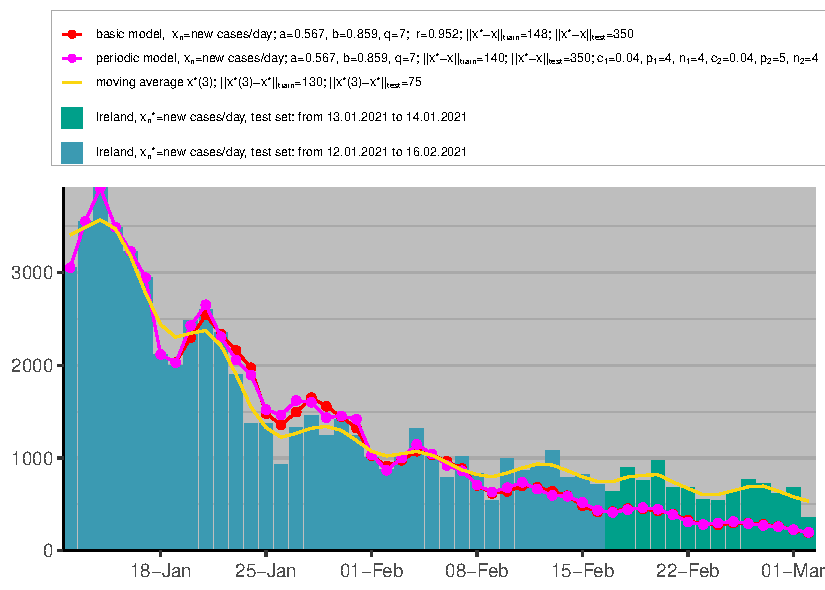
\includegraphics[width=\linewidth]{Ireland-periodic-traintest.pdf} \label{fig:ireland-periodic-traintest}
\endminipage\hfill
\minipage{0.48\textwidth}
  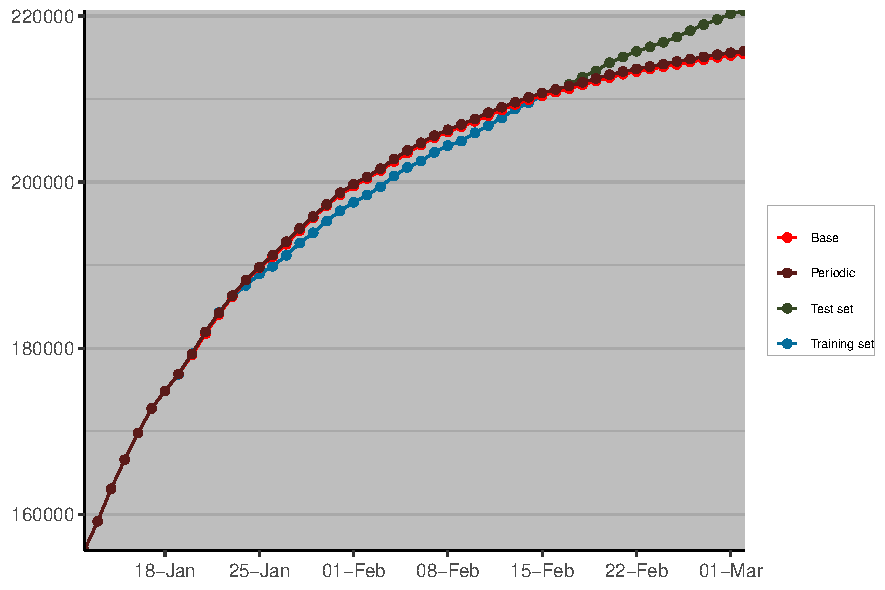
\includegraphics[width=\linewidth]{Ireland-periodicy-traintest.pdf} \label{fig:ireland-periodicy-traintest}
\endminipage
\caption{Periodic model with train/test split, Ireland}
\end{figure}

\begin{figure}[H]
\minipage{0.48\textwidth}
  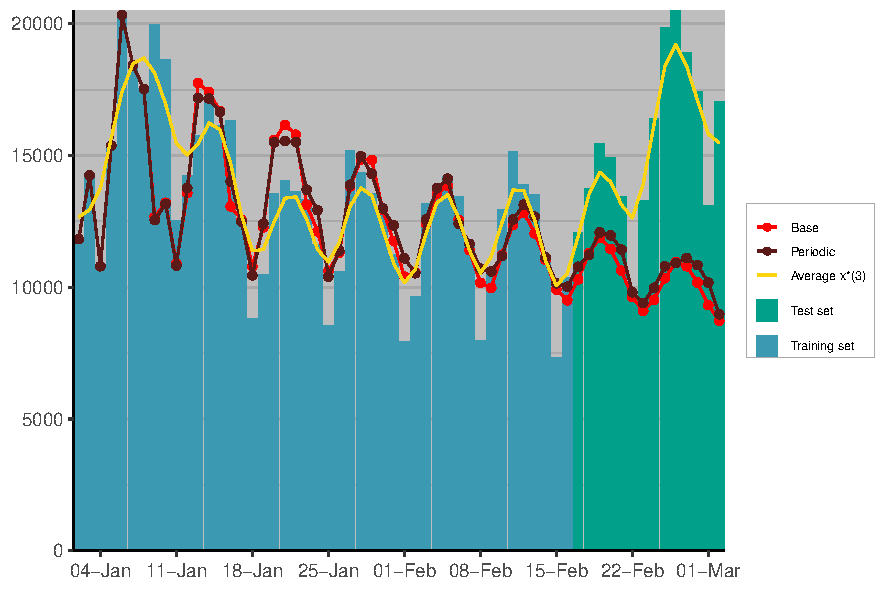
\includegraphics[width=\linewidth]{Italy-periodic-traintest.pdf} \label{fig:italy-periodic-traintest}
\endminipage\hfill
\minipage{0.48\textwidth}
  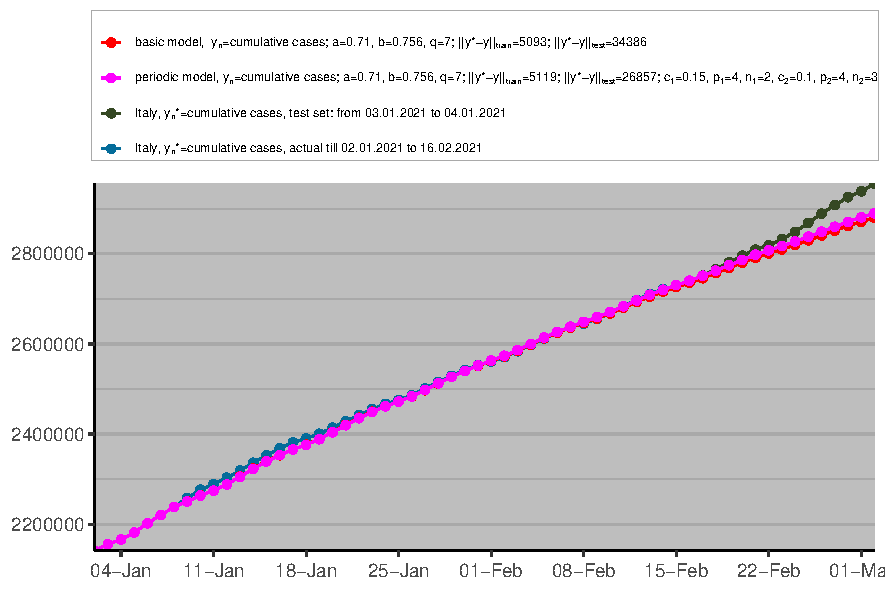
\includegraphics[width=\linewidth]{Italy-periodicy-traintest.pdf} \label{fig:italy-periodicy-traintest}
\endminipage
\caption{Periodic model with train/test split, Italy}
\end{figure}

\begin{figure}[H]
\minipage{0.48\textwidth}
  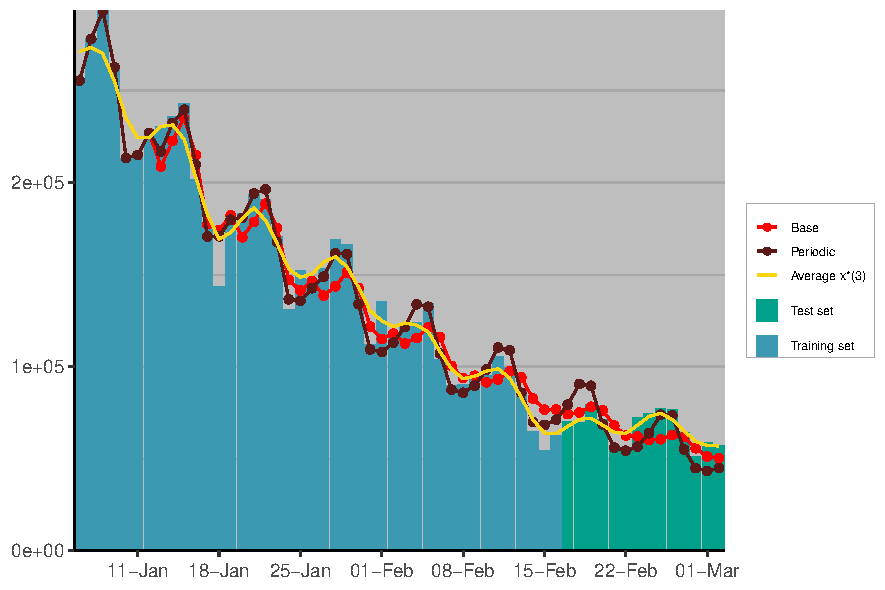
\includegraphics[width=\linewidth]{United States-periodic-traintest.pdf} \label{fig:us-periodic-traintest}
\endminipage\hfill
\minipage{0.48\textwidth}
  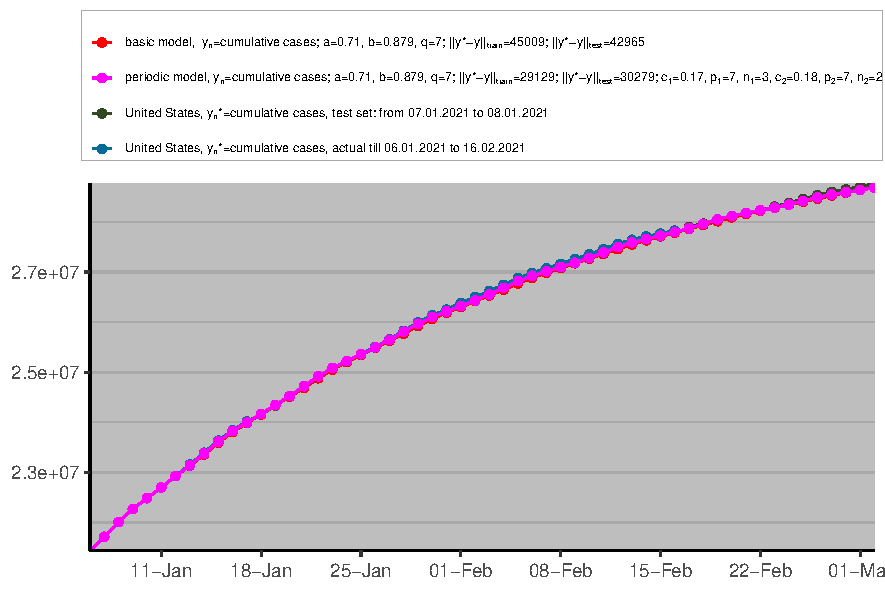
\includegraphics[width=\linewidth]{United States-periodicy-traintest.pdf} \label{fig:us-periodicy-traintest}
\endminipage
\caption{Periodic model with train/test split, United States}
\end{figure}

\subsection{HoltWinters model}
\begin{figure}[H]
\minipage{0.48\textwidth}
  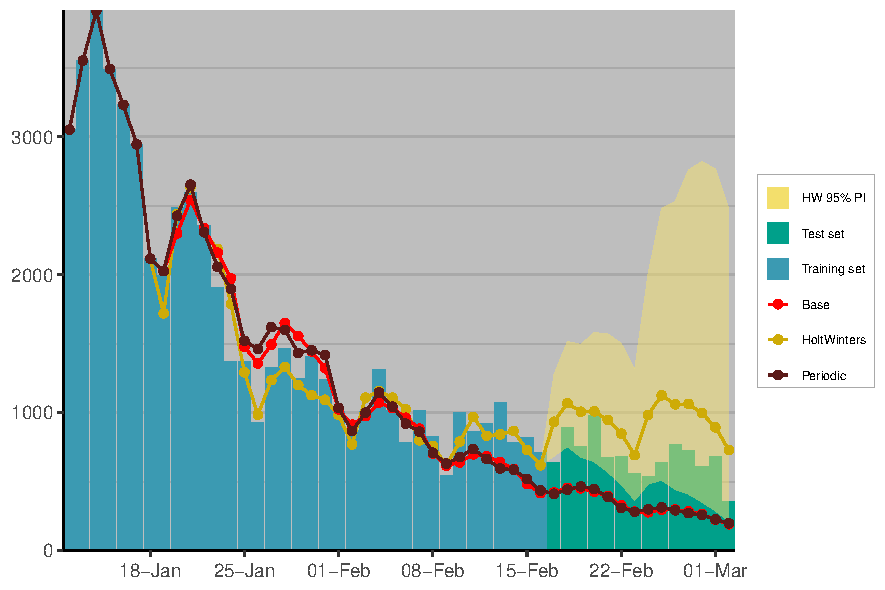
\includegraphics[width=\linewidth]{Ireland-hw-traintest.pdf} \label{fig:ireland-hw-traintest}
\endminipage\hfill
\minipage{0.48\textwidth}
  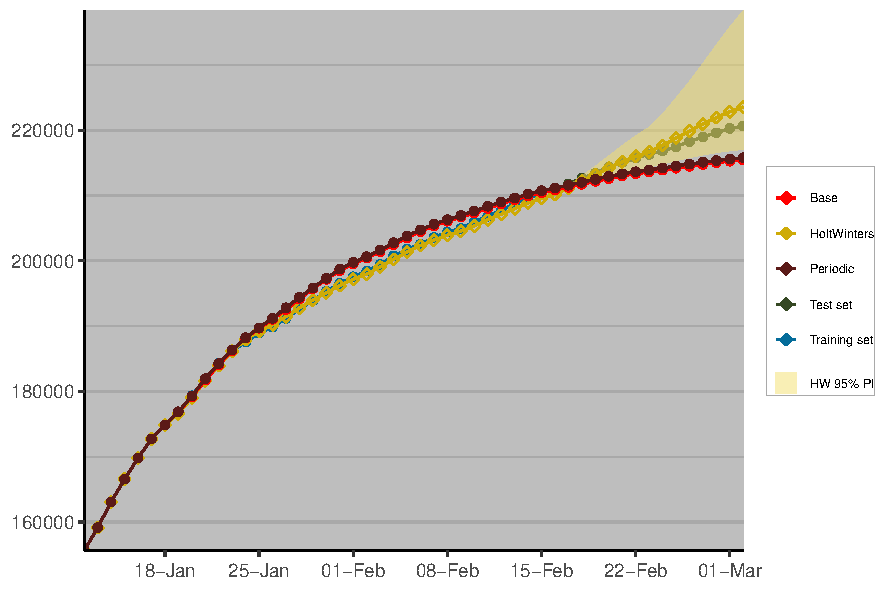
\includegraphics[width=\linewidth]{Ireland-hwy-traintest.pdf} \label{fig:ireland-hwy-traintest}
\endminipage
\caption{HoltWinters model with train/test split, Ireland}
\end{figure}

\begin{figure}[H]
\minipage{0.48\textwidth}
  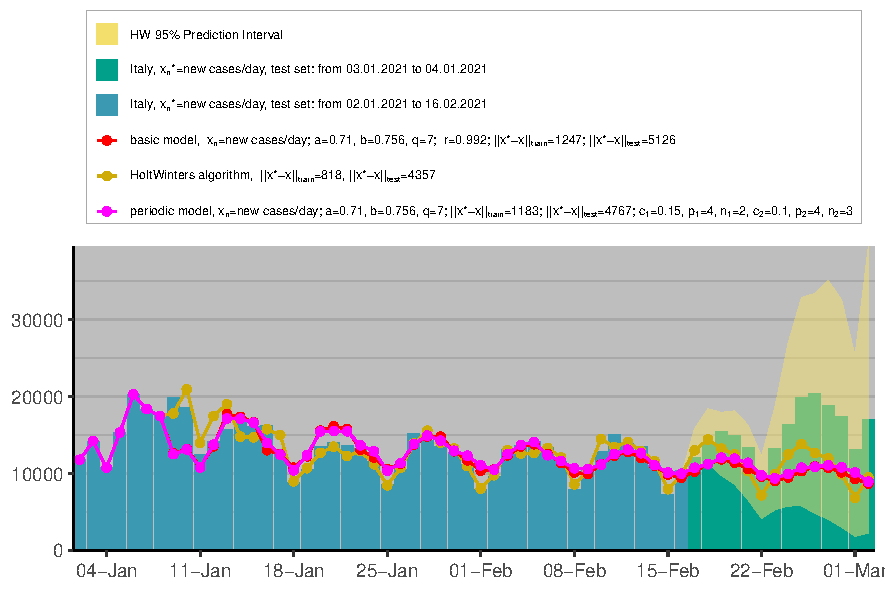
\includegraphics[width=\linewidth]{Italy-hw-traintest.pdf} \label{fig:italy-hw-traintest}
\endminipage\hfill
\minipage{0.48\textwidth}
  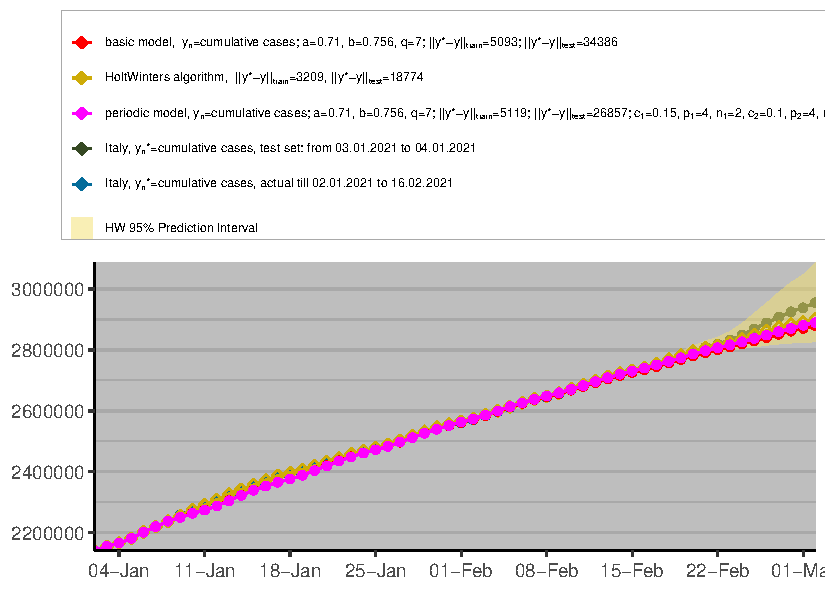
\includegraphics[width=\linewidth]{Italy-hwy-traintest.pdf} \label{fig:italy-hwy-traintest}
\endminipage
\caption{HoltWinters model with train/test split, Italy}
\end{figure}

\begin{figure}[H]
\minipage{0.48\textwidth}
  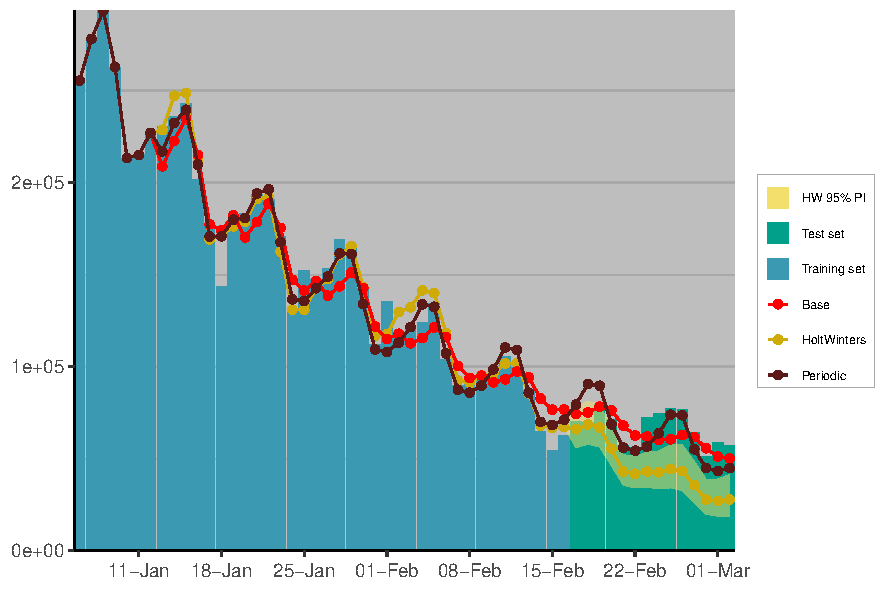
\includegraphics[width=\linewidth]{United States-hw-traintest.pdf} \label{fig:us-hw-traintest}
\endminipage\hfill
\minipage{0.48\textwidth}
  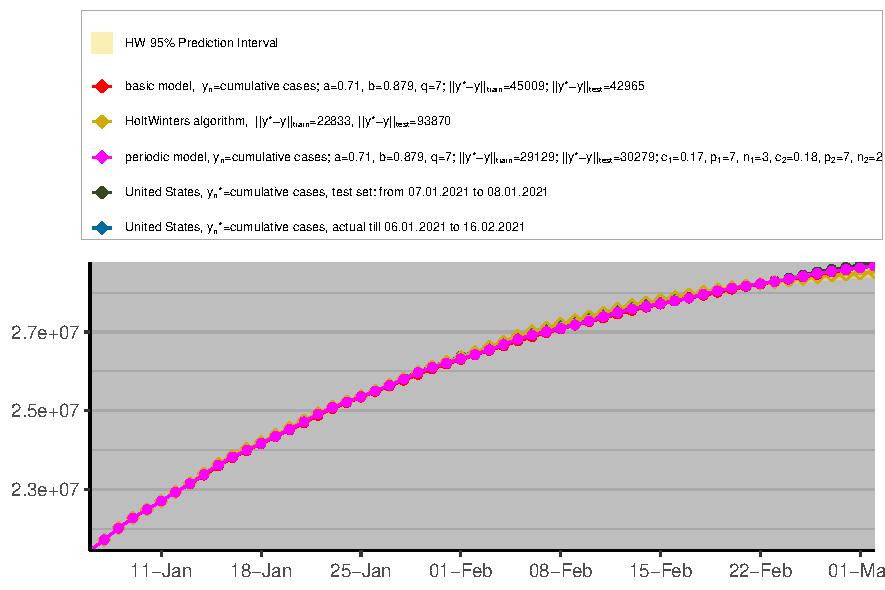
\includegraphics[width=\linewidth]{United States-hwy-traintest.pdf} \label{fig:us-hwy-traintest}
\endminipage
\caption{HoltWinters model with train/test split, United States}
\end{figure}

\subsection{ARIMA model}
\begin{figure}[H]
\minipage{0.48\textwidth}
  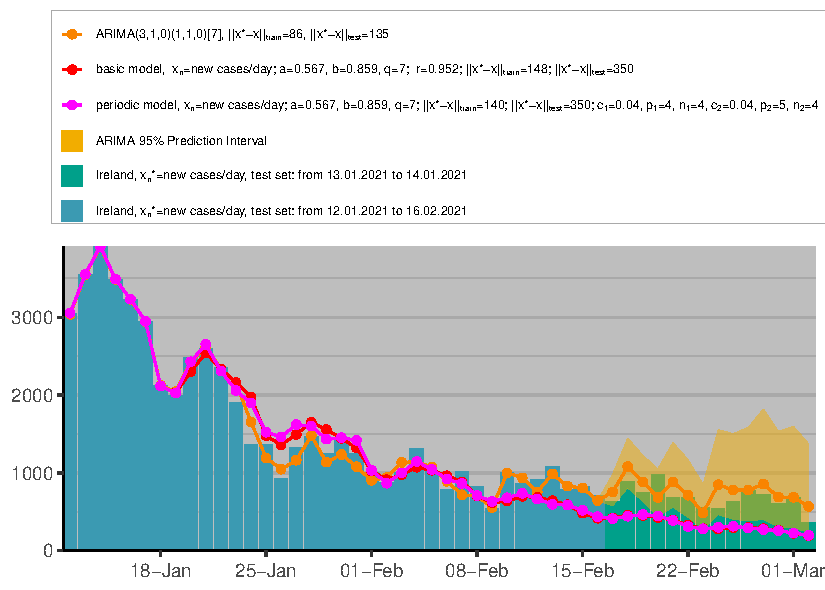
\includegraphics[width=\linewidth]{Ireland-arima-traintest.pdf} \label{fig:ireland-arima-traintest}
\endminipage\hfill
\minipage{0.48\textwidth}
  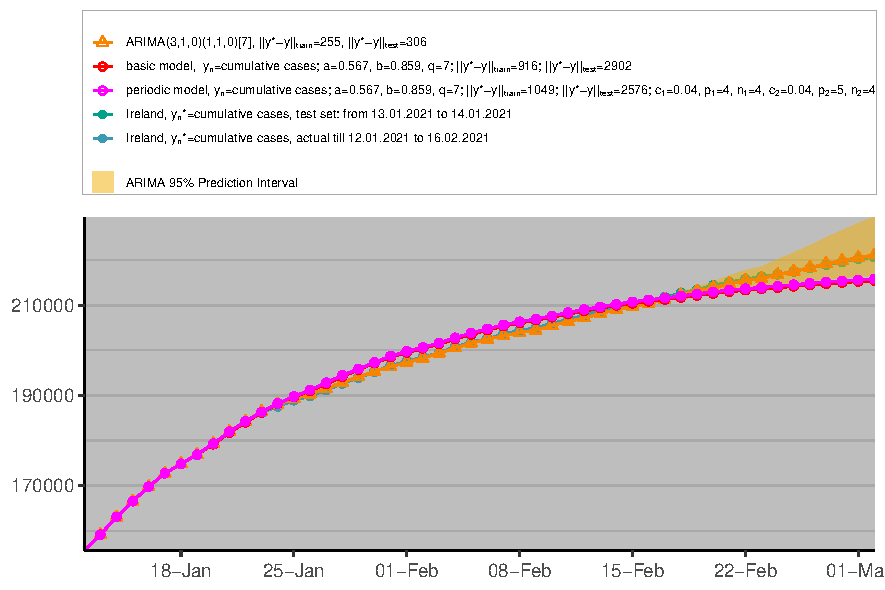
\includegraphics[width=\linewidth]{Ireland-arimay-traintest.pdf} \label{fig:ireland-arimay-traintest}
\endminipage
\caption{ARIMA model with train/test split, Ireland}
\end{figure}

\begin{figure}[H]
\minipage{0.48\textwidth}
  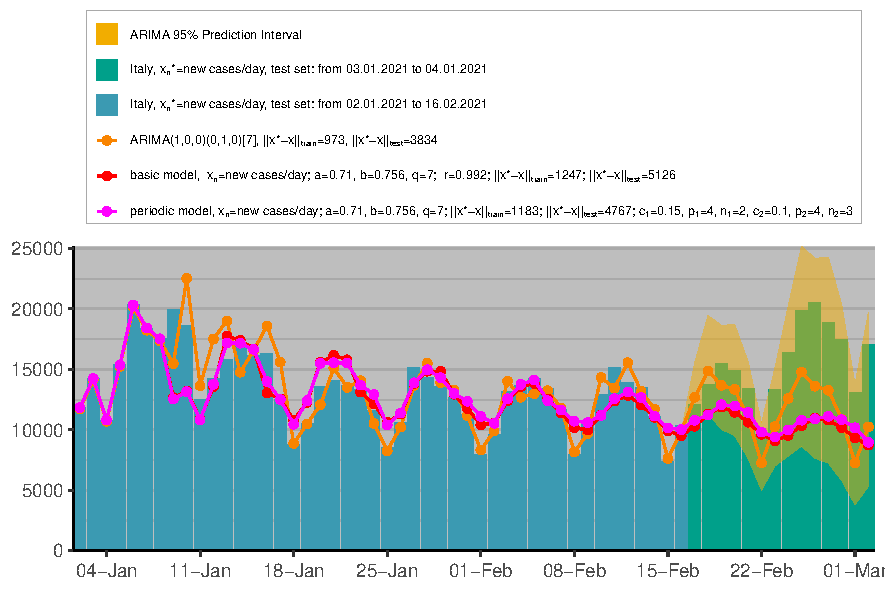
\includegraphics[width=\linewidth]{Italy-arima-traintest.pdf} \label{fig:italy-arima-traintest}
\endminipage\hfill
\minipage{0.48\textwidth}
  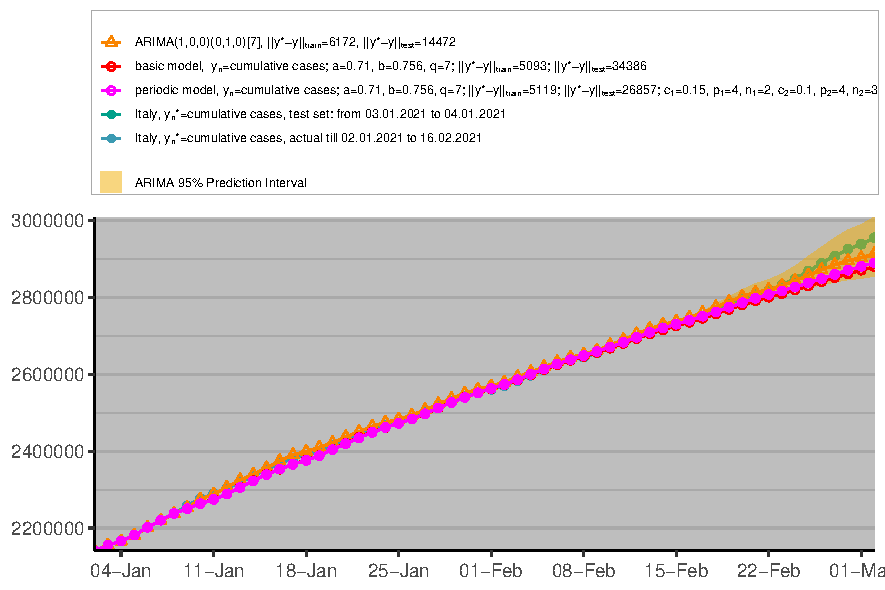
\includegraphics[width=\linewidth]{Italy-arimay-traintest.pdf} \label{fig:italy-arimay-traintest}
\endminipage
\caption{ARIMA model with train/test split, Italy}
\end{figure}

\begin{figure}[H]
\minipage{0.48\textwidth}
  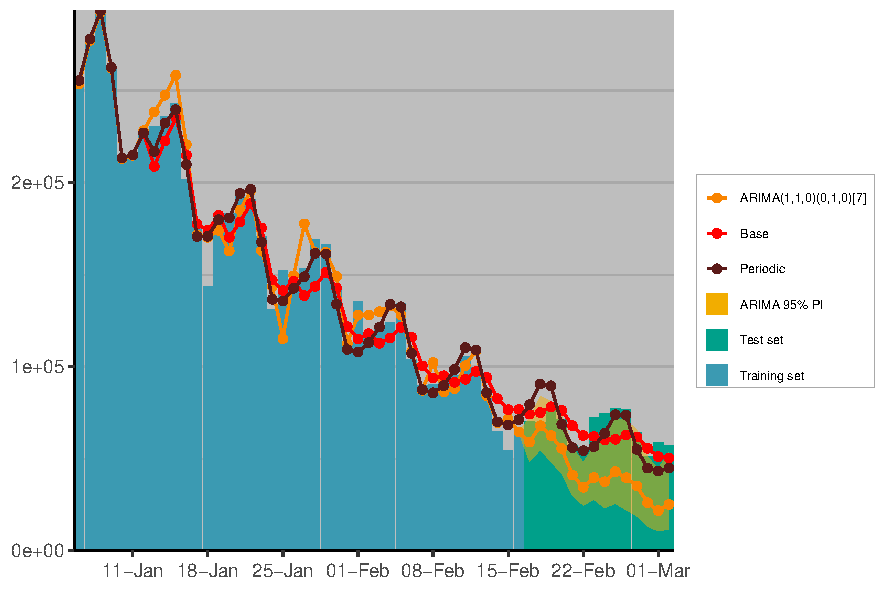
\includegraphics[width=\linewidth]{United States-arima-traintest.pdf} \label{fig:us-arima-traintest}
\endminipage\hfill
\minipage{0.48\textwidth}
  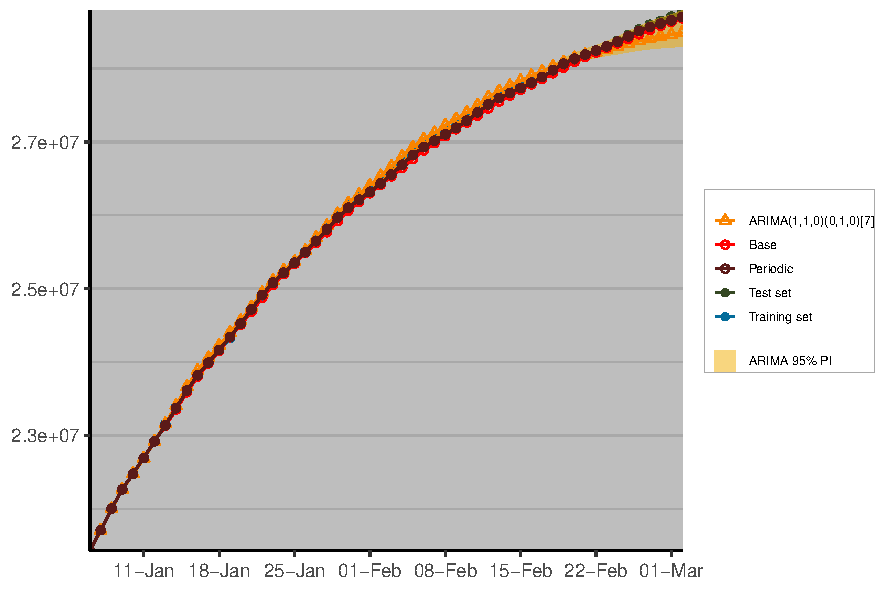
\includegraphics[width=\linewidth]{United States-arimay-traintest.pdf} \label{fig:us-arimay-traintest}
\endminipage
\caption{ARIMA model with train/test split, United States}
\end{figure}

\subsection{NNAR model}
\begin{figure}[H]
\minipage{0.48\textwidth}
  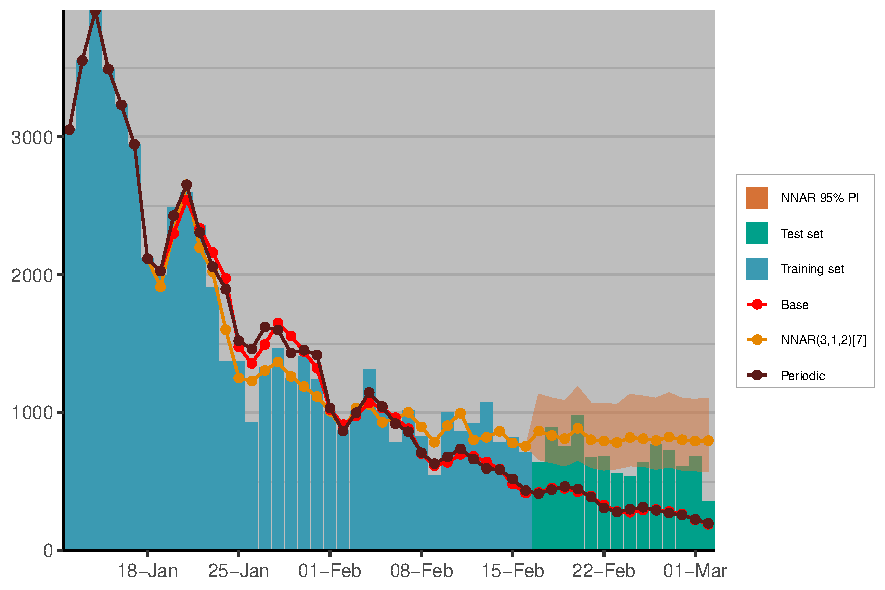
\includegraphics[width=\linewidth]{Ireland-nn-traintest.pdf} \label{fig:ireland-nn-traintest}
\endminipage\hfill
\minipage{0.48\textwidth}
  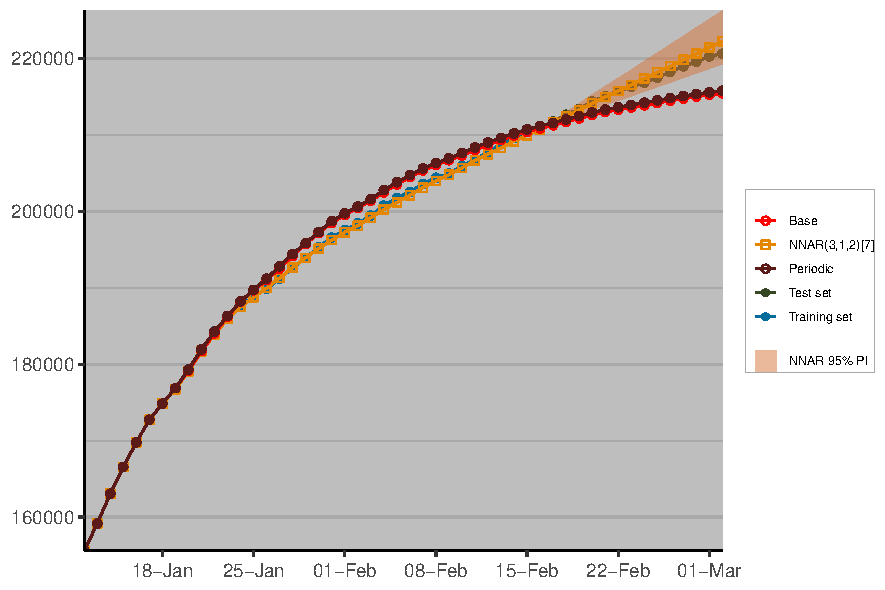
\includegraphics[width=\linewidth]{Ireland-nny-traintest.pdf} \label{fig:ireland-nny-traintest}
\endminipage
\caption{Neural Network Autoregression model with train/test split, Ireland}
\end{figure}

\begin{figure}[H]
\minipage{0.48\textwidth}
  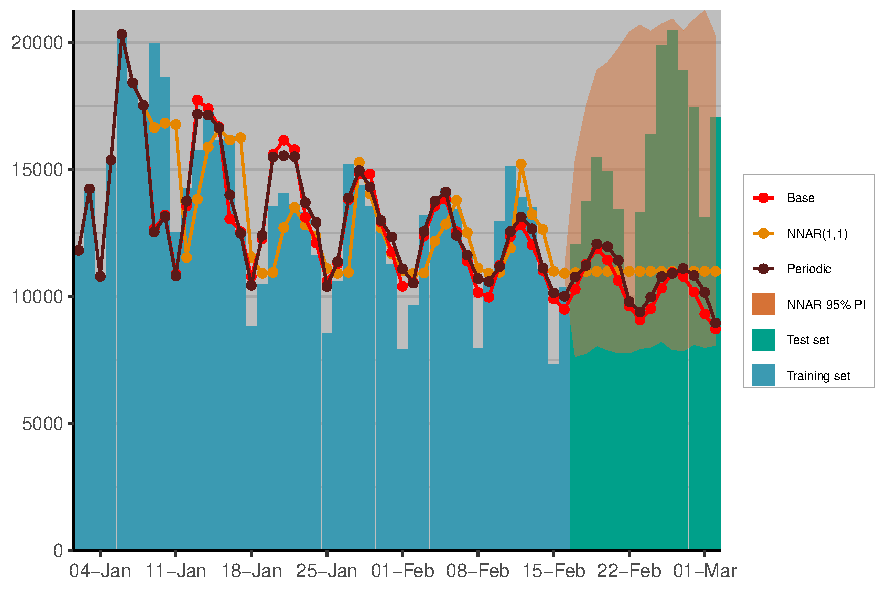
\includegraphics[width=\linewidth]{Italy-nn-traintest.pdf} \label{fig:italy-nn-traintest}
\endminipage\hfill
\minipage{0.48\textwidth}
  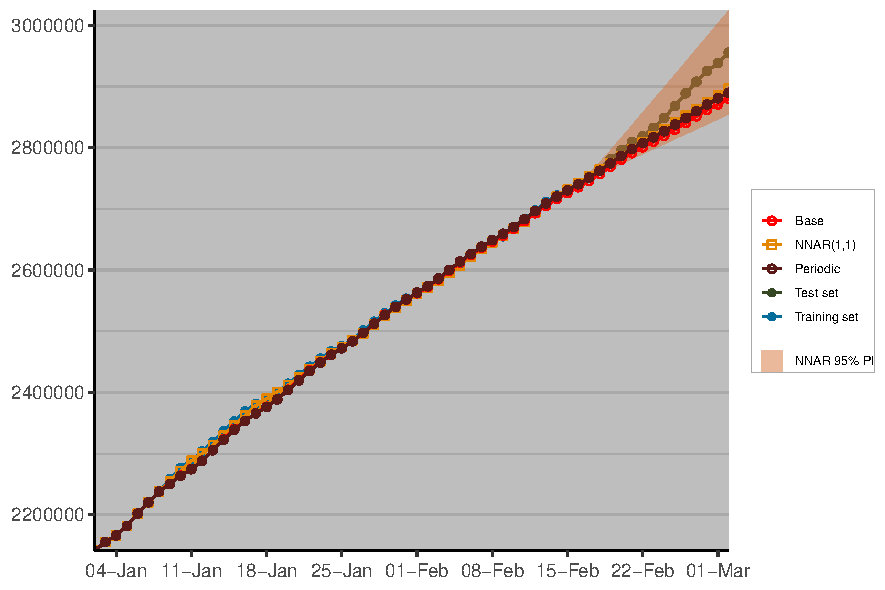
\includegraphics[width=\linewidth]{Italy-nny-traintest.pdf} \label{fig:italy-nny-traintest}
\endminipage
\caption{Neural Network Autoregression model with train/test split, Italy}
\end{figure}

\begin{figure}[H]
\minipage{0.48\textwidth}
  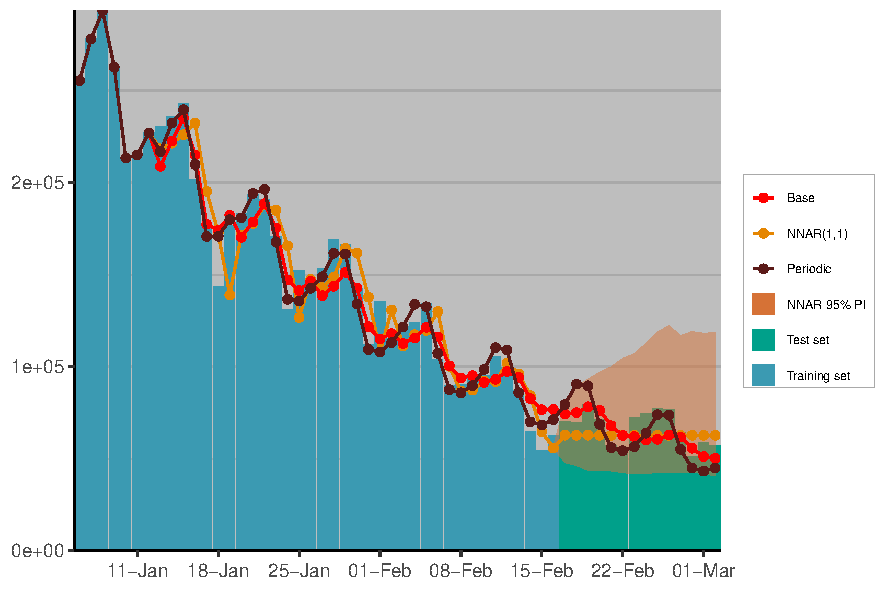
\includegraphics[width=\linewidth]{United States-nn-traintest.pdf} \label{fig:us-nn-traintest}
\endminipage\hfill
\minipage{0.48\textwidth}
  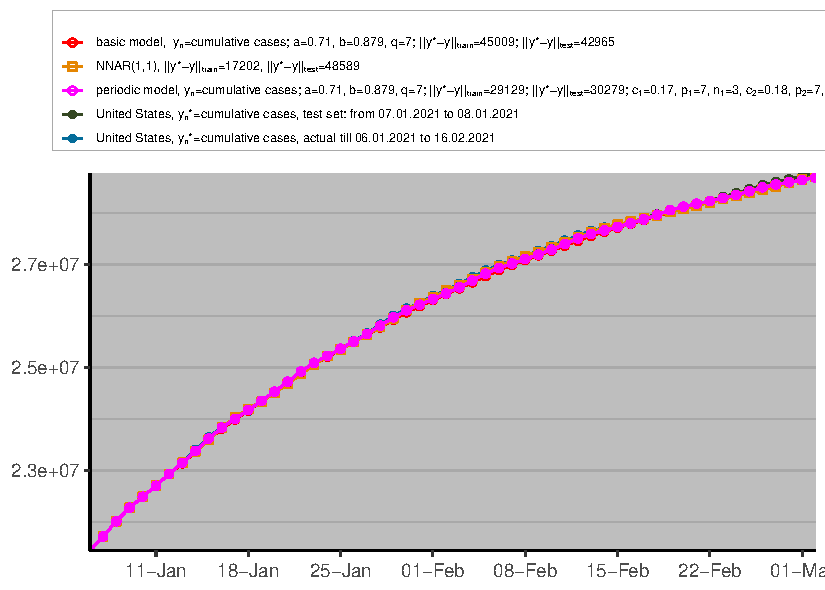
\includegraphics[width=\linewidth]{United States-nny-traintest.pdf} \label{fig:us-nny-traintest}
\endminipage
\caption{Neural Network Autoregression model with train/test split, United States}
\end{figure}